\section{Синтез структуры синхронного автомата Мура}

\subsection{Постановка задачи}

Синтезировать структурную схему синхронного цифрового автомата Мура 
с входом в виде меандровой последовательности, 4-я состояниями памяти 
и двумя выходами, включающими: на первом выходе автомата состояния памяти на первом и третьем шаге, 
на втором выходе – на втором и четвертом шаге работы автомата в цикле.

Состояния памяти автомата в каждом очередном такте поступления синхросигнала изменяется по данному циклу: 11, 10, 01, 00. 
Начальное состояние памяти автомата: 00.

\subsection{Алгоритм синтеза структурного автомата}

Алгоритм метода канонического структурного синтеза автомата состоит в следующем:
%
\begin{enumerate}
    \item Закодировать состояния памяти автомата.
    \item Закодировать входные и выходные сигналы автомата.
    \item Выбрать элементы памяти автомата.
    \item Построить уравнения функций переходов и выходов автомата.
    \item Синтезировать структурную схему автомата.
    \item Конец алгоритма.
\end{enumerate}

\vspace{1em}

Так как состояния памяти и входные/выходные сигналы закодированы,
выполнение пунктов алгоритма 1 - 3 не требуется.

\subsection{Построение граф-схемы работы автомата}

На рисунке \ref{fig:task5:graph} изображена граф-схема данного автомата.

\begin{figure}[h!]
    \centering
    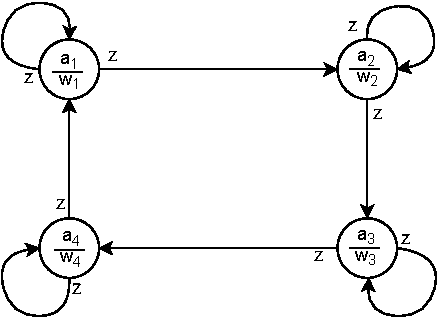
\includegraphics[scale=1]{S5IM1.pdf}
    \caption{Граф-схема автомата Мура}
    \label{fig:task5:graph}
\end{figure}

\subsection{Выбор элементов памяти автомата}

Рассмотрим состояния памяти автомата в порядке их изменения во времени: 00, 11, 10, 01.

Данная последовательность образует конечную циклическую группу двухразрядных двоичных чисел
с образующей 11:
%
\begin{equation*}
    C = (A, \Sigma)
\end{equation*}

\begin{explanation}
    \item[где] $A = \{00, 11, 10, 01\}$ - носитель алгебры;
    \item $\Sigma = \{\oplus\}$ - сигнатура алгебры, операция сложения по модулю 2.
\end{explanation}

\vspace{1em}

Так как последовательность состояний памяти образует циклическую группу, 
переход состояния памяти можно записать следующим образом:
%
\begin{equation*}
    a^{*} = a \oplus 11.
\end{equation*}
%
Соответствующие уравнения переходов для каждого разряда состояния памяти имеют вид:
%
\begin{equation*}
    {a_0}^{*} = {a_0} \oplus 1,
\end{equation*}
%
\begin{equation*}
    {a_1}^{*} = {a_1} \oplus 1 \oplus {a_0} \wedge 1 = {a_1} \oplus (a_0 \oplus 1) = {a_1} \oplus \bar{a_0}.
\end{equation*}

Наиболее подходящим типом элемента памяти для данных уравнений переходов является T-триггер, 
так он меняет свое состояние по принципу сложения по модулю 2.

\subsection{Построение функций переходов}

Построим таблицу переходов внутреннего состояния памяти автомата 
с соответствующими для этих переходов значениями функции возбуждения элементов памяти.

\begin{table}[h!]
    \caption{Таблица переходов автомата}
    \begin{tabular}{| >{\centering}m{0.05\textwidth} 
                    | >{\centering}m{0.05\textwidth}
                    | >{\centering}m{0.05\textwidth}
                      >{\centering}m{0.05\textwidth}  
                    | >{\centering}m{0.05\textwidth} 
                      >{\centering}m{0.05\textwidth} 
                    | >{\centering}m{0.05\textwidth} 
                      >{\centering\arraybackslash}m{0.05\textwidth}|} 
        \hline
            $t$ & ${x}$ & ${A_1}$ & ${A_2}$ & ${A_1}^{*}$ & ${A_2}^{*}$ & ${T_1}$ & ${T_2}$ \\
        \hline\multirow{2}*{1} 
            &   1   &    0    &    0    &      1      &      1      &    1    &    1    \\
        \cline{2-8}
            &   0   &    1    &    1    &      1      &      1      &    0    &    0    \\
        \hline\multirow{2}*{2} 
            &   1   &    1    &    1    &      1      &      0      &    0    &    1    \\
        \cline{2-8}
            &   0   &    1    &    0    &      1      &      0      &    0    &    0    \\
        \hline\multirow{2}*{3} 
            &   1   &    1    &    0    &      0      &      1      &    1    &    1    \\
        \cline{2-8}
            &   0   &    0    &    1    &      0      &      1      &    0    &    0    \\
        \hline\multirow{2}*{4} 
            &   1   &    0    &    1    &      0      &      0      &    0    &    1    \\
        \cline{2-8}
            &   0   &    0    &    0    &      0      &      0      &    0    &    0    \\
        \hline
    \end{tabular}
    \label{tab:task5:table1}
\end{table}

Из таблицы \ref{tab:task5:table1} получим уравнения функций возбуждения элементов памяти:
%
\begin{equation}
    T_1 = x\bar{A_2} 
    \label{eq:task5:T1}
\end{equation}
%
\begin{equation}
    T_2 = x
    \label{eq:task5:T2}
\end{equation}

\subsection{Построение функций выходов}

По условию задачи автомат имеет 2 выхода. 
Первый выход $Y_1$ содержит значения памяти автомата на первом и третьем тактах работы автомата, 
а второй выход $(Y_2)$ -- на втором и четвертом. 

Значения на выходе, не задействованном на данном такте, будем считать отрицательно определенными.

Построим таблицу зависимости выходов $Y_1(y_1, y_2)$, $Y_2(y_3, y_4)$ от состояния памяти автомата $(A_1, A_2)$.

\begin{table}[h!]
    \caption{Таблица выходных сигналов автомата}
    \begin{tabular}{| >{\centering}m{0.05\textwidth} 
                    | >{\centering}m{0.05\textwidth}
                    | >{\centering}m{0.05\textwidth}
                    | >{\centering}m{0.05\textwidth}  
                    | >{\centering}m{0.05\textwidth} 
                    | >{\centering}m{0.05\textwidth} 
                    | >{\centering\arraybackslash}m{0.05\textwidth}|} 

        \hline $t$ & ${A_1}$ & ${A_2}$ & ${y_1}$ & ${y_2}$ & ${y_3}$ & ${y_4}$ \\
        \hline  1  &    0    &    0    &    0    &    0    &    0    &    0    \\
        \hline  2  &    1    &    1    &    0    &    0    &    1    &    1    \\
        \hline  3  &    1    &    0    &    1    &    0    &    0    &    0    \\
        \hline  4  &    0    &    1    &    0    &    0    &    0    &    1    \\
        \hline
    \end{tabular}
    \label{tab:task5:table2}
\end{table}

Из таблицы \ref{tab:task5:table2} получим уравнения функций выходных сигналов автомата:
%
\begin{equation}
    y_1 = {A_1}\bar{A_2} 
    \label{eq:task5:Y1}
\end{equation}
%
\begin{equation}
    y_2 = 0
\end{equation}
%
\begin{equation}
    y_3 = {A_1}{A_2}
\end{equation}
%
\begin{equation}
    y_4 = {A_2}
    \label{eq:task5:Y4}
\end{equation}

\subsection{Синтез структурной схемы автомата}

На основе данных, полученных в предыдущих подразделах, синтезируем структурную схему автомата Мура.

Комбинационная схема перехода цифрового автомата задается уравнениями (\ref{eq:task5:T1}), (\ref{eq:task5:T2}).

Комбинационная схема выхода цифрового автомата задается уравнениями (\ref{eq:task5:Y1}) - (\ref{eq:task5:Y4}).

В качестве элементов памяти внутреннего состояния автомата используются Т-триггеры.

Выходной сигнал $y_2$ не зависит от внутреннего состояния автомата и является постоянным: $y_2 = const = 0$.

На рисунке \ref{fig:task5:scheme} изображена синтезированная структурная схема исходного автомата.

\begin{figure}[h!]
    \centering
    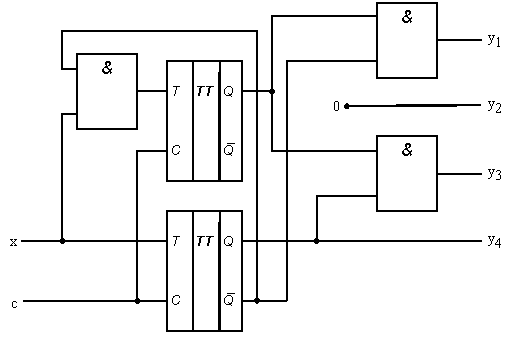
\includegraphics[scale=1.4]{S5IM2.pdf}
    \caption{Структурная схема автомата Мура}
    \label{fig:task5:scheme}
\end{figure}